\chapter{Fonctionnalité implémentées}

\section{Les annotations}

Nous avons implémenté différentes annotations qui sont 
incrustables sur des vidéos. Si on lance l'exécutable de 
\textbf{annotateImage}, les choix d'annotations se font seulement
avant le lancement du programme.

Ces choix se font dans le fichier
\textit{annotation\_settings.json}.
Si on lance l'interface, les choix d'affichage s'initialisent
grâce au fichier Json mais peuvent être modifiés pendant la
lecture de la vidéo. 
Nous allons suivre l'architecture du fichier Json pour expliquer
les différentes fonctionnalités implémentées pour les
annotations.
\bigskip

Le booléen "write" présent pour chaque annotation exprime
l'écriture ou non sur l'image de l'annotation.
\bigskip

Il faut également récupérer les numéros des équipes. Soit ils
sont connus, soit il faut les récupérer avec l'exécutable
\textit{init\_match} du package annotateImage
explique~\ref{init}, page~\pageref{init}.


\subsection{Les couleurs}

Les deux premiers éléments du fichier json sont la couleurs de 
chaque équipe. Par défaut, les couleurs des équipes sont bleu 
pour l'équipe 1 et rose pour l'équipe 2, ce qui correspond aux 
couleurs des robots en match.

\newpage

\subsection{La position}

La position permet d'afficher un cercle montrant la position où 
le robot pense être.
Elle s'affiche forcément pour tous les robots à la fois ou aucun.
Il est possible de choisir le rayon du cercle (en pixel) et
l'affichage ou non du numéro du robot au centre de la position. 
\bigskip

La taille de l'écriture du numéro est proportionnelle à 
$\frac{3}{4}$ du rayon du cercle. Il est donc déconseillé de 
l'afficher si la taille du cercle est minime.

La position s'affiche simplement en transformant le point du plan
réel en point sur l'image grâce à la fonction \textbf{fieldToImg}
fournie par le client.

\subsection{La direction}

L'annotation de la direction dessine une flèche montrant la 
direction vers laquelle le robot avance. La flèche démarre de la 
position du robot. Il est possible de changer sa taille.

\bigskip

La flèche est créée en définissant un second point sur le dessin 
dans la direction donnée (en radian). Ce point est déterminé en 
additionnant les coordonnées de la position à $\cos$(direction) 
pour l'axe des $x$ et $\sin$(direction) pour l'axe des  $y$.

Ensuite, nous transposons nos deux points dans le plan de l'image
grâce à \textbf{fieldToImg}.

Enfin, nous calculons la distance entre ce nouveau point et la
position grâce au théorème de Pythagore, puis nous réduisons
proportionnellement cette distance à la taille de la flèche
souhaitée.
\bigskip

Nous affichons la flèche de la couleur de l'équipe du robot. Il 
se peut que la flèche s'affiche en noir, cela signifie que 
l'angle donné par le robot est supérieur $2*\Pi$. Ceci témoigne 
d'une imprécision du robot. 
Nous pouvons voir cette erreur dans la vidéo 2vs1.


\begin{figure}[h] 
\centering 
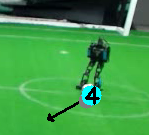
\includegraphics[scale = 0.5]{images/wrongdir.png}
    \caption{Erreur de direction d'un robot}
    \label{fig:dir}
\end{figure}

\newpage

\subsection{La trace}

L'annotation de la trace est représentée par de multiples cercles
modélisant les anciennes positions du robot. 
La trace ne peut être visible que sur un robot à la fois, il peut
être changé en cours de match lorsque la visualisation est lancée
avec l'interface. 
\bigskip

Elle s'affiche de la couleur de l'équipe du Robot choisi mais en
plus foncé comme on peut le voir dans la Figure~\ref{fig:trace}.
Nous pouvons choisir la taille de la trace, il est préférable de 
l'avoir plus petite que la position.


La trace nous montre les dernières positions depuis un certain 
nombre de secondes définit dans \textit{annotation\_settings} 
grâce à "delay\_old\_pos". La trace est stockée dans une map.
\bigskip

Pour afficher la trace nous affichons donc toutes les positions 
présentes dans la map pour un certain nombre de secondes 
précédentes.
\bigskip

\begin{figure}[h] 
\centering 
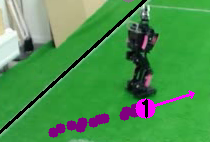
\includegraphics[scale = 0.5]{images/robottrace.png}
    \caption{Affichage de la trace}
    \label{fig:trace}
\end{figure}

\subsection{La balle}

Tout comme la trace, nous ne pouvons voir la balle du point de 
vue que d'un seul robot à la fois. Nous pouvons choisir la taille
de la balle. La couleur de la balle est définie arbitrairement en
gris.
\bigskip

Ce qui a été compliqué avec la balle c'est que la position de la 
balle est donnée dans le repère du robot, non du terrain. 

En effet, dans les logs (Figure~\ref{fig:message}), la position 
du robot est définie grâce \textit{self\_in\_field} donc dans le 
repère du terrain mais la position de la balle est dans 
\textit{ball\_in\_self} donc d'après le repère du robot.
\bigskip

Nous avons donc du changer de repère grâce à une équation de 
plan.
\newpage
Soit ($x_B$, $y_B$) les coordonnées de la balle dans le repère du
robot et ($x_B$',$y_B$') dans le repère du terrain. On définit 
également ($x_R$, $y_R$) les coordonnées du robot dans le plan du
terrain et $\theta$ l'angle de la direction du robot en radian. 

L'équation est donc :
\bigskip

\[\left\{
  \begin{array}{ccccccc}
    x_B'& =& x_R &+& x_B \cos(\theta)& - & y_B \sin(\theta)\\
    y_B' &= & x_R &+& x_B \sin(\theta)& +& y_b \cos(\theta)\\
  \end{array}
\right.
\]    

\subsection{La position souhaitée (Target)}

La target représente la position que le robot souhaite atteindre.
Elle ne s'affiche donc que pour un robot à la fois.
\bigskip

Elle est marquée par une croix dont la taille est définie par
l'utilisateur dans "target\_size". Si on a également la position
du robot, une ligne en pointillé s'affiche entre la position du
robot et celle souhaitée. 
Il est possible de ne pas afficher cette ligne en mettant un
nombre plus grand que la taille de l'image (avec les vidéos
données, 1000 convient parfaitement).
\bigskip

La taille des traits est égale à la taille des espaces, pour
tracer la ligne, nous avons fait un itérateur qui colorise un
certain nombre de pixel pour le trait puis qui laisse l'espace de
même taille.


\begin{figure}[h] 
\centering 
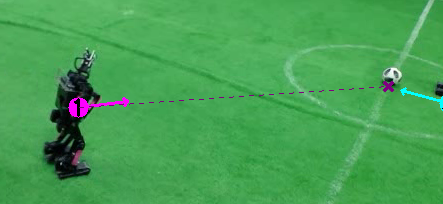
\includegraphics[scale = 0.5]{images/robottarget.png}
    \caption{Affichage de la target}
    \label{fig:target}
\end{figure}
\newpage


\subsection{Les lignes du terrain et le score}

Nous pouvons choisir d'afficher les lignes du terrain en
fournissant le fichier Json définissant les caractéristiques du
terrain sur lequel le match est joué. La fonction d'affichage des
lignes a été fournie par le client.
Ce fichier Json est nécessaire pour la calibration de la caméra.
\bigskip

Comme nous en avons vu Figure~\ref{fig:field} à la
page~\pageref{fig:field}, les lignes du terrain peuvent parfois
avoir des erreurs à cause de la distorsion de la caméra.

Afficher ces lignes peut nous aider à comprendre les différences
entre la position annotée et réelle du robot.
\bigskip

Il y a une possibilité d'afficher le score dans un des coins de
l'écran. Les valeurs à donner en x et y sont données en
commentaire dans le Json. Nous n'avons pas défini de coin par
défaut car il peut changer à chaque vidéo. Par exemple, l'idéal
pour la vidéo static de 2vs1 est dans le coin en haut à gauche
mais si on l'affiche là, le score ne se voit pas sur la vidéo
webcam du 21/03/2019.
\bigskip

Il faut noter que le score s'affiche automatiquement dans
l'interface.

\subsection{Délai et optimisation des annotations}

Les deux derniers éléments du fichier Json sont
"delay\_annotation" et "optimized". Le premier exprime le temps
en seconde durant lequel un message est considéré comme valide.
C'est à dire le temps pour lequel on va l'afficher avant qu'il
soit trop vieux.

\bigskip

L'optimisation permet d'afficher les annotations avec une opacité
reflétant la durée. Un message plus vieux sera plus transparent
qu'un message tout juste reçu. 
\bigskip

\label{transparence}
Pour l'ajout de certaines annotations comme la trace, nous avons
souhaité utiliser la transparence.
Ainsi, les anciennes positions deviennent graduellement
transparentes, jusqu'à disparaître.


\begin{figure}[h] 
\centering 
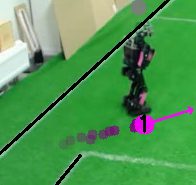
\includegraphics[scale = 0.5]{images/traceoptimized.png}
    \caption{Affichage de la trace optimisé}
    \label{fig:trace_opti}
\end{figure}



Nous avons donc décidé d'utiliser la fonction d'OpenCV
(\textbf{AddWeighted}) permettant de fusionner deux images en
fonction d'une opacité.

\bigskip
\newpage
La transparence des objets se fait en trois étapes.
\bigskip

Tout d'abord, on calcule l'opacité en fonction du temps.
\bigskip

Ensuite on copie l'image dans une image provisoire (overlay) et
on ajoute l'annotation à cette copie. Ensuite on ajoute l'image
copiée et annotée à l'image de départ (blend) en fonction de
l'opacité calculée grâce à la fonction OpenCV. 

\bigskip

La différence de performance entre les annotations non optimisées
et optimisées est calculée dans les tests sur la performance
en~\ref{testperf}, page~\pageref{testperf}.

\section{Les outils de annotateImage}

En dehors des tests, nous avons deux fichiers exécutables dans la
partie annotateImage.

\subsection{Init\_match} \label{init}


Tous les choix sur les numéros de robot et d'équipe peuvent être
difficiles si on ne connaît pas les robots de la vidéo. 
L'exécutable \textit{init\_match} permet de lire les 30 premières
secondes de vidéo et de connaître donc les robots présent en jeu
ainsi que leur équipe. On peut en voir le résultat
Figure~\ref{fig:init_match} :

\begin{figure}[h] 
\centering 
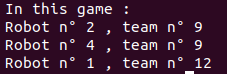
\includegraphics[scale = 0.5]{images/init_match.png}
    \caption{Résultat de l'exécutable init\_match}
    \label{fig:init_match}
\end{figure}


Tout comme les tests, il faut activer les tools de
\textbf{annotateImage} dans le CMakeList pour avoir l'exécutable
\textit{init\_match}.


\subsection{Main\_annotateImage}

Notre fichier principal de lancement est l'outil
\textit{main\_annotateImage}.

Il permet de lancer un monitoring et d'afficher une vidéo
simplement, comme cela a été détaillé dans l'architecture du
projet.
\bigskip

Il y a une option ajustable pour le fichier
\textit{main\_annotateImage} dans le fichier de configuration
\textit{match\_settings}. Il s'agit de l'élément
"speed\_optimized". Si, l'utilisateur met ce booléen à false,
alors le match défilera le plus vite possible pour l'ordinateur.
Sinon, le match défilera à vitesse normale, c'est à dire à la
même vitesse que le fichier vidéo fourni.
\bigskip

Pour cela, nous calculons le temps réel écoulé depuis le
lancement de la vidéo grâce à deux chronos. Nous comparons
ensuite ce temps écoulé au temps écoulé de la vidéo.
\bigskip

Si nous avons de l'avance par rapport à la vidéo alors nous
ralentissons grâce à un temps d'attente avant la prochaine image.

Sinon nous passons immédiatement à l'image suivante. En cas de
retard trop important, nous sautons une image ce qui nous permet
de ne pas avoir de retard par rapport à la vidéo.

\section{L'interface}


Nous ajoutons des annotations sur une vidéo de match. Cependant,
étant donné le grand nombre d'informations, l'image peut se
trouver saturée et devenir illisible. Notre interface doit
résoudre ce problème en proposant des options d'affichage qui
conviennent à différents usages.
\bigskip

\subsection{Choix de l'API}

Dans un premier temps, il a fallu choisir une API pour créer
l'interface de notre programme. Nous en cherchions une plutôt
facile à prendre en main, en C++, et qui propose suffisamment
d'options pour créer une interface complète. 
\bigskip

Nous avons d'abord pensé à \textbf{OpenCV}, que nous utilisons
déjà pour les annotations. La prise en main est assez rapide mais
les options sont trop peu nombreuses. Les interfaces en
\textbf{OpenCV} se limitent principalement à afficher des images,
sans aspect esthétique. 

\bigskip

\textbf{GTK} et \textbf{FLTK} ont été rapidement considérés, mais
la prise en main semblait trop compliquée et aurait pris trop de
temps. 

\bigskip

Nous avons donc choisit \textbf{QT} dans sa version 5.9, qui est
très bien documenté \cite{ref4}, facile à prendre en main et
présente un très large éventail d'options pour créer une
interface riche et complète.

\bigskip

Au début du projet, nous avons rencontré des difficultés pour
faire communiquer l'interface et les fonctions d'annotation.
Après la refonte de l'architecture du projet, la liaison entre
les modules interfaces et \textbf{annotateImage} était grandement
simplifiée, et nous avons pu lire une vidéo dans notre fenêtre
\textbf{Qt}. 
\bigskip

Nous avons ensuite pu ajouter des options pour choisir les
annotations à afficher, modifiables pendant la lecture de la
vidéo. 
\bigskip

De chaque coté de la vidéo, nous affichons des informations sur
le match, les robots, les équipes et les choix d'annotations.
\bigskip

\subsection{Affichage de la vidéo}

On ne peut pas afficher d'image cv$::$Mat dans un label d'une
interface QT. Ce format d'image est toutefois celui nécessaire
pour les annotations. Nous convertissons donc l'image produite
par nos fonctions de traitement en QImage, puis en QPixmap. Elle
est ensuite placée dans le label idoine.

\bigskip

Pour rafraîchir l'image, un Qtimer fait appel à la fonction
\textbf{changeImage} avec un intervalle de \textit{SPD\_INTERVAL}
millisecondes. Cette fonction reprend le fonctionnement de
\textit{main\_annotateImage}, mais au lieu d'afficher la vidéo de
sortie, les images sont placées dans \textbf{labelVideo}. 


\subsection{Les fonctionnalités de l'interface}

Lorsque nous lançons l'interface, la configuration des
annotations par défaut sera lu dans le fichier
\textit{annotation\_settings.json}.


Nous voyons alors s'afficher la fenêtre d'interface comme 
ci-dessous.
\newpage


\begin{figure}[h] 
\centering 
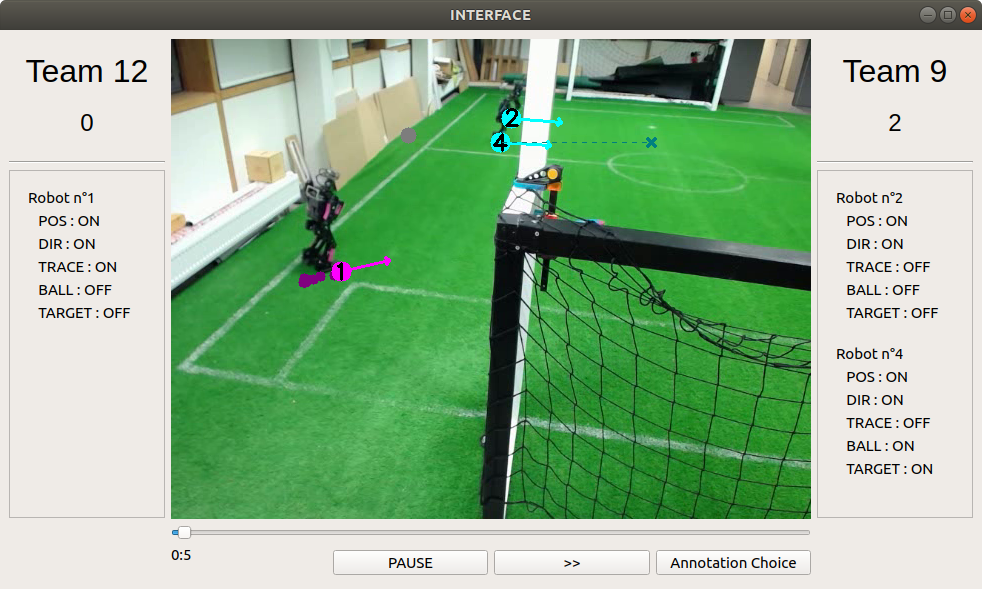
\includegraphics[scale = 0.35]{images/interface.png}
\caption{Fenêtre d'interface}
\label{fig:interface}
\end{figure}

Les deux panneaux à droite et à gauche de la vidéo sont créés
grâce aux classes \textbf{TeamPanel} et \textbf{RobotPanel}.
Ils contiennent les informations sur les annotations en cours.
\bigskip

En dessous de la vidéo, nous avons le slider expliqué un peu plus
bas, partie~\ref{slider}.
\bigskip

Ensuite, nous avons les 3 boutons de l'interface. 

Le premier est un simple bouton play/pause qui permet de faire
des arrêts sur image. (Très pratique par exemple pour prendre des
situations en photos, voir Figure~\ref{fig:dir})
\bigskip

Le second bouton est un bouton FastForward permettant de changer
la vitesse d'affichage de la vidéo.

Au démarrage, la vidéo est en 30ms/img, une vitesse normale. En
activant le bouton $\gg$, la vitesse de la vidéo passe à 1ms/img,
c'est-à-dire que la vitesse de la vidéo est régulée par la
vitesse des annotations.

C'est l'équivalent du booléen \textit{speed\_optimized} de
\textit{match\_settings} nous permettant de faire varier la
vitesse de la vidéo dans le fichier \textit{main\_annotateImage}.
\bigskip

Enfin, le dernier bouton permet de faire apparaître une fenêtre
pop-up permettant de changer les annotations 
(Figure~\ref{fig:annot}).

\begin{figure}[h] 
\centering 
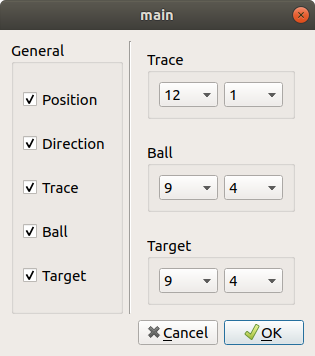
\includegraphics[scale = 0.35]{images/annotationchoice.png}
\caption{Fenêtre de choix d'annotations}
\label{fig:annot}
\end{figure}

Nous voyons que les robots affichés pour les annotations sont les
mêmes que ceux de la vidéo.

\subsection{Le slider} \label{slider}

Un slider a été implémenté pour choisir un moment précis de la
vidéo. Il prend des valeurs allant de 0 à 99. 
\bigskip

Pour que le slider avance automatiquement lorsque la vidéo est en
lecture, on calcule le pourcentage d'avancement à partir du
\textit{time\_stamp} de l'image actuelle et de la durée totale de
la vidéo.
\bigskip

Lorsque le slider est déplacé, le \textit{time\_stamp}
correspondant à l'image et aux messages à lire est incrémenté
(respectivement décrémenté) jusqu'à atteindre la position
indiquée par le slider. Seul un entier est modifié dans une
boucle while, nous ne parcourons pas toutes les images et
messages entre les deux \textit{time\_stamp}. Pour l'utilisateur,
la latence est donc négligeable. 
\bigskip

La position maximale du slider est donc 99, ce qui correspond
donc à 99\% de la vidéo. Il reste donc encore 1\% de à lire à ce
moment.
\bigskip

On affiche le temps écoulé dans un label en dessous du slider. Ce
temps est exprimé en minutes et secondes. Les matchs ne devraient
pas durer une heure, notamment à cause de la batterie des robots.

Il nous a semblé plus pertinent de simplifier l'affichage en
ayant seulement deux nombres (minutes et secondes) plutôt qu'un
nombre pour les heures qui serait égal à 0 dans la majorité des
cas. Si le match dure plus de 60 minutes, le nombre de minute
continuera d'incrémenter.
\bigskip

Arrivé à la fin de la vidéo, ce n'est plus le temps qui s'affiche
mais "end of video".
\bigskip